% !TEX program = pdflatex
\documentclass[12pt,a4paper]{report}

% Packages
\usepackage[utf8]{inputenc}
\usepackage[T1]{fontenc}
\usepackage{geometry}
\usepackage{graphicx}
\usepackage{fancyhdr}
\usepackage{titlesec}
\usepackage{tocloft}
\usepackage{xcolor}
\usepackage{hyperref}
\usepackage{enumitem}
\usepackage{caption}
\usepackage{float}
\usepackage{tikz}
\usepackage{amsmath}
\usepackage{listings}
\usepackage{fontawesome5}
\usepackage{setspace}

% listings styling
\lstset{
    basicstyle=\ttfamily\scriptsize,
    breaklines=true,
    frame=single,
    backgroundcolor=\color{lightgray},
    keywordstyle=\color{primaryblue}\bfseries,
    commentstyle=\color{green!60!black},
    stringstyle=\color{orange},
    numbers=left,
    numberstyle=\tiny\color{gray},
    stepnumber=1,
    showstringspaces=false,
    tabsize=2
}

% Page geometry
\geometry{
    left=1.5in,
    right=1in,
    top=1in,
    bottom=1in
}

% Colors
\definecolor{primaryblue}{RGB}{41, 98, 255}
\definecolor{darkgray}{RGB}{51, 51, 51}
\definecolor{lightgray}{RGB}{245, 245, 245}

% Hyperref setup
\hypersetup{
    colorlinks=true,
    linkcolor=primaryblue,
    filecolor=primaryblue,
    urlcolor=primaryblue,
    citecolor=primaryblue,
    pdftitle={Job Nova Documentation},
    pdfauthor={},
    pdfsubject={SaaS Platform Documentation},
    pdfkeywords={job, Digital Platform}
}

% Chapter formatting
\titleformat{\chapter}[display]
{\normalfont\huge\bfseries\color{primaryblue}}
{\chaptertitlename\ \thechapter}{20pt}{\Huge}

\titlespacing*{\chapter}{0pt}{-20pt}{40pt}

% Section formatting
\titleformat{\section}
{\normalfont\Large\bfseries\color{primaryblue}}
{\thesection}{1em}{}

\titleformat{\subsection}
{\normalfont\large\bfseries\color{darkgray}}
{\thesubsection}{1em}{}

% Header and footer
\pagestyle{fancy}
\fancyhf{}
\fancyhead[L]{\leftmark}
\fancyhead[R]{\thepage}
\fancyfoot[C]{Job Nova}
\renewcommand{\headrulewidth}{0.5pt}
\renewcommand{\footrulewidth}{0.5pt}

% Custom list markers
\setlist[itemize,1]{label=\textbullet}
\setlist[itemize,2]{label=\textendash}

% Document begins
\begin{document}

% Title page
\begin{titlepage}


\begin{center}
            \centering
            \vspace{1cm}

            % HEADER
            {\large \textbf{\textit{\underline{Project Report On}}}}
            
            \vspace{0.5cm}

            % TITLE
            {\Huge \textbf{Job Nova}}
            
            \vspace{0.5cm}

            % SUBMISSION STATEMENT
            {\large \textbf{A dissertation partial fulfillment of all the requirements of MCA
Degree of the Maulana Abul Kalam Azad
University Of Technology for the year 2024-25}}

            \vspace{0.5cm}

            
            \includegraphics[width=3.5cm, height=3.5cm, keepaspectratio]{college logo transparent.png} 
            
            \vspace{0.5cm}

            % SUBMITTED BY SECTION
            {\Large \textbf{Submitted By}}
            
            \vspace{0.5cm}
            
            {\large \textbf{Dipankar Shaw(26371024013)}\\[5pt]
            \textbf{Asif Shohood(26371024010)}\\[5pt]
            \textbf{Ananta Mondal(26371024051)}\\[5pt]
            \textbf{Abhranil Das(26371024042)}}

            \vspace{1cm}

            % GUIDANCE SECTION
            {\large \textbf{Under the guidance of}\\[5pt]
            \Large \textbf{Ms. Debalina Barman}\\[5pt]
            \large \textbf{Project guide}\\[5pt]
            \textbf{Dept of Master of Computer Application}\\
            \textbf{Regent Education \& Research Foundation Group of Institutes}}

            \vspace{0.5cm}

            % LOGO 2 (MAKAUT / Utech)
            % Replace 'makaut_logo.png' with your actual image file
            % \includegraphics[width=2.5cm]{makaut_logo.png}
             % Placeholder for the code to compile without the image:
            \includegraphics[width=2.5cm, height=2.5cm, keepaspectratio]{MAKAUAT_LOGO.png}

            \vspace{0.2cm}

            % FOOTER
            {\small \textbf{(Affiliated to the Maulana Abul Azad University of Technology, formerly\\
            known as West Bengal University of Technology , West Bengal)\\
            Barrackpore, KOLKATA - 700121}}
            
            \vspace{1cm}
 
\end{center}

\end{titlepage}

\pagenumbering{roman} 

\begin{center}
            \centering
            \vspace{0.5cm}

            % --- HEADER SECTION ---
            % Using columns to place Logo on left and Text on right
            \begin{minipage}{0.18\textwidth}
                \includegraphics[width=\linewidth]{college logo transparent.png} % Placeholder
            \end{minipage}%
            \hfill
            \begin{minipage}{0.78\textwidth}
                \centering
                {\textbf{REGENT EDUCATION AND RESEARCH FOUNDATION GROUP OF INSTITUTES}}
            \end{minipage}

            \vspace{0.5cm}

            % --- TITLE ---
            {\Large \textbf{\underline{Certificate of Approval}}}

            \vspace{0.5cm}

            % --- BODY TEXT ---
            \parbox{0.95\textwidth}{
                \onehalfspacing
                \large
                This is to certify that this report of MCA final year project, Job Nova is a record of bona-fide work, carried out by \textbf{Dipankar Shaw, Asif Shohood , Ananta Mondal \& Abhranil Das} under my supervision and guidance.

                \vspace{1em}

                In my opinion, the report in its present form is in partial fulfillment of all the requirements, as specified by Regent Education And Research Foundation Group of Institutes and as per regulation of the \textbf{Maulana Abul Kalam Azad University Of Technology}. In fact, it has standard, necessary for submission to the best of my knowledge, the content embodied in this report, are original in nature and worthy for incorporation in the present version of the report for MCA program.
            }

            \vspace{1.5cm}

            % --- GUIDE SIGNATURE ---
            Guide/supervisor

            \vspace{1.5cm}
            
            \rule{8cm}{0.5pt} \\ % Horizontal Line
            \textbf{Ms. Debalina Barman} \\[5pt]
            Department of Master of Computer Application\\
            Regent Education \& Research Foundation Group of Institutes

            \vspace{2cm}

            % --- EXAMINER & HOD SIGNATURES ---
            \noindent
            \begin{minipage}[t]{0.45\textwidth}
                \centering
                \rule{6cm}{0.5pt}\\
                \textbf{Examiner(s)}
            \end{minipage}%
            \hfill
            \begin{minipage}[t]{0.45\textwidth}
                \centering
                \rule{7cm}{0.5pt}\\
                \textbf{Head of the Department}\\[5pt]
                \textbf{Master of Computer Application}
            \end{minipage}

            \vfill % Pushes the footer to the bottom
\vspace{0.25cm}
            % --- FOOTER ---
            \hrule % Horizontal line separating footer
        \vspace{0.25cm}
            
            {\scriptsize \textbf{Campus: Regent Education \& Research Foundation Group of Institutions}\\}
          
            
            {\tiny \textbf{Address: Bara Kanthalia (Barrackpore), Post: Sewli Telinipara, P.S.: Titagarh, Kolkata-700 121 \\Tel.: 033 2535-3051/3053 Fax: 033 2535-3460}\\}
          
            
            {\tiny \textbf{Regd. Office: 88, Chowringhee Road, Kolkata-700 020 E-mail: \underline{rerfkolkata@gmail.com} \\Website: \underline{www.rerf.com}}\\}
            
        
            
            {\tiny \textbf{City Office: 3rd Floor, 60B, Chowringhee Road, Kolkata 700 020, Tel: (+91 33) 2290 0112/13/14 , \\Fax No.: 033-2290-0}}
            
           
   
\end{center}

\newpage


\begin{center}
            \centering
            \vspace{3cm}

            % --- TITLE ---
            {\Huge \textbf{\textcolor{primaryblue}{DECLARATION}}}

            \vspace{2.5cm}

            % --- BODY TEXT ---
            \parbox{0.95\textwidth}{
                \onehalfspacing
                \large
                We, \textbf{Dipankar Shaw} (Reg. No. 242630510014), \textbf{Asif Shohood} (Reg. No. 242630510009), \textbf{Ananta Mondal} (Reg. No. 242630510005), and \textbf{Abhranil Das} (Reg. No. 242630510003), hereby declare that the project report entitled ``\textbf{Job Nova}'' is the outcome of our own work and has been carried out under the guidance of \textbf{Ms. Debalina Barman}, Assistant Professor, Department of MCA.

                \vspace{1em}

                This project is submitted in partial fulfillment of the requirements for the award of the \textbf{Master of Computer Applications (MCA)} degree.

                \vspace{1em}
                
                We also declare that this report has not been submitted to any other institution or university for the award of any degree, diploma, or certificate
            }

            \vspace{2cm}

            % --- SIGNATURE SECTION ---
            \begin{flushright}
                \large \textbf{\textit{Date and Signature}}\hspace{1cm}
            \end{flushright}
            
            \vspace{0.5cm}

            % Using a table for alignment of names and signature lines
            \noindent
            \begin{tabular}{p{0.5\textwidth} p{0.4\textwidth}}
                \textbf{\large Dipankar Shaw(26371024013)} & \rule{7cm}{0.5pt} \\[1.5cm]
                \textbf{\large Asif Shohood(26371024010)} & \rule{7cm}{0.5pt} \\[1.5cm]
                \textbf{\large Ananta Mondal(26371024051)} & \rule{7cm}{0.5pt} \\[1.5cm]
                \textbf{\large Abhranil Das(26371024042)} & \rule{7cm}{0.5pt} \\
            \end{tabular}

            \vfill % Pushes the footer to the bottom
            \vspace{5pt}
            % --- FOOTER ---
            \hrule % Horizontal line separating footer
          
            \vspace{5pt}
            \centering
            {\scriptsize \textbf{Campus: Regent Education \& Research Foundation Group of Institutions}\\}
            {\tiny \textbf{Address: Bara Kanthalia (Barrackpore), Post: Sewli Telinipara, P.S.: Titagarh, Kolkata-700 121 Tel.: 033 2535-3051/3053 Fax: 033 2535-3460}\\}
            
            {\tiny \textbf{Regd. Office: 88, Chowringhee Road, Kolkata-700 020 E-mail: \underline{rerfkolkata@gmail.com} Website: \underline{www.rerf.com}}\\}
            
            {\tiny \textbf{City Office: 3rd Floor, 60B, Chowringhee Road, Kolkata 700 020, Tel: (+91 33) 2290 0112/13/14 , Fax No.: 033-2290-0}}
            
\end{center}


\begin{center}
            
            \centering
            \vspace{3cm} % Top padding inside box

            % TITLE
            {\Huge \textbf{\textcolor{primaryblue}{ACKNOWLEDGEMENT}}} 
            
            \vspace{2.5cm} % Space between title and text

            % BODY TEXT
            % Using a parbox to slightly indent the text block relative to the border
            \parbox{\linewidth}{ 
                \setlength{\parskip}{1.5em} % Space between paragraphs
                \onehalfspacing             % Line spacing
                \large                      % Font size
                
                I  would like to take this opportunity to express my heartfelt gratitude to \textbf{Ms. Debalina Barman}, Assistant Professor, Department of MCA, and \textbf{Mr. Krishna Kanta Maiti}, Assistant Professor and Head of the Department, for their continuous support, expert guidance, and constant encouragement throughout the duration of this project.
                
Their unwavering support, insightful feedback, and valuable suggestions have been a source of
motivation and have significantly contributed to the successful completion of this project. 
Their dedication to teaching and commitment to student development are truly inspiring, and I am extremely grateful for the opportunity to work under their guidance.

I am also deeply thankful to all the teaching and non-teaching staff members of the Department of
Masters in Computer Application for their assistance, cooperation, and moral support throughout the project. Their help in various administrative and technical aspects ensured the smooth progress of my work.

Lastly, I would like to thank my fellow classmates and friends for their constant encouragement,
valuable discussions, and positive spirit, which made this journey more enriching and enjoyable.
This project has been a great learning experience, and I am truly thankful to everyone who contributed directly or indirectly to its successful completion.
            }
\end{center}

\newpage

% Abstract
\begin{center}
            
            \centering
            \vspace{3cm} % Top padding inside box

            % TITLE
            {\Huge \textbf{\textcolor{primaryblue}{ABSTRACT}}} 
            
            \vspace{2.5cm} % Space between title and text

            % BODY TEXT
            % Using a parbox to slightly indent the text block relative to the border
            \parbox{\linewidth}{ 
                \setlength{\parskip}{1.5em} % Space between paragraphs
                \onehalfspacing             % Line spacing
                \large                      % Font size
                
                JobNova is an AI-based job recommendation system designed to simplify the recruitment process for both job seekers and employers. Traditional job portals often provide generic job listings, making it difficult for candidates to find positions that match their skills and interests. JobNova addresses this issue by using intelligent algorithms to analyze user profiles, skills, qualifications, and preferences to recommend relevant job opportunities. The system provides secure user authentication, resume management, job posting, job application tracking, and personalized recommendations. Employers can efficiently post vacancies, manage applications, and shortlist suitable candidates, while job seekers can search and apply for jobs with ease. The platform is developed using modern web technologies to ensure high performance, scalability, and an intuitive user experience. By integrating artificial intelligence into the recruitment process, JobNova reduces the time required for job searching and candidate selection while improving the accuracy of job recommendations. The proposed system aims to bridge the gap between employers and job seekers by providing an efficient, reliable, and user-friendly recruitment platform.
            }
\end{center}

\newpage

% Table of contents
\tableofcontents
\cleardoublepage        % or \clearpage
\pagenumbering{arabic}
\setcounter{page}{1}
\newpage


% Chapter 2: Introduction
\chapter{INTRODUCTION}

\section{Background}

In the contemporary professional landscape, the recruitment process serves as a vital bridge between human talent and organizational growth. In a country as vast and competitive as India, both private corporations and public sector enterprises are constantly searching for efficient hiring mechanisms. However, traditional job boards and manual recruitment processes are increasingly fragmented and inefficient. Job seekers are forced to navigate dozens of platforms, manually construct and format static resumes, and submit applications into dark pools where they receive little to no feedback. Concurrently, recruiters are overwhelmed by hundreds of unstandardized applications, making manual resume screening a major bottleneck that is both time-consuming and prone to cognitive fatigue and bias.

\section{Problem Statement}

The existing recruitment methodology presents several key pain points for both candidates and employers:
\begin{itemize}
    \item \textbf{Inadequacy of Static Resumes}: A traditional static CV fails to convey a candidate's verbal communication skills, interactive problem-solving capabilities, or domain-specific enthusiasm.
    \item \textbf{High Screening Overhead}: Recruiters must manually filter, read, and evaluate hundreds of applications for every open position. This leads to extended hiring cycles and missed talent.
    \item \textbf{Fragmented Public Sector Listings}: In the Indian job market, public sector (government) job announcements are scattered across hundreds of disparate departmental web portals, making it extremely difficult for job seekers to track deadlines, eligibility, and vacancies.
    \item \textbf{Lack of Interactive Career Guidance}: Job seekers rarely receive personalized, interactive feedback on their profiles or structured preparation assistance for interviews.
\end{itemize}

\section{Proposed Solution: JobNova}

To overcome these challenges, we developed \textbf{JobNova} --- an AI-driven, serverless recruitment platform tailored specifically to modernize hiring. JobNova leverages local Large Language Models (LLMs) and serverless edge databases to automate the onboarding, screening, and job discovery processes.

Unlike traditional recruitment portals, JobNova provides:
\begin{itemize}
    \item \textbf{Conversational AI Onboarding}: Instead of filling out dense forms, job seekers build their profiles by chatting with an interactive AI assistant. The AI dynamically extracts contact info, academic details, and professional experience, structured as JSON.
    \item \textbf{AI Job Agent}: A personalized career assistant that answers queries, analyzes jobseeker profiles, recommends matching positions, and automates application procedures.
    \item \textbf{Automated AI Applicant Screening}: For jobs with AI screening enabled, applicants complete a short, interactive screening chat. The AI evaluates their responses, calculates a matching score, and provides a concise summary to the employer.
    \item \textbf{Government Jobs Portal}: A built-in scraping engine collects public sector openings, presenting them in a unified interface to streamline search and compliance tracking.
\end{itemize}

\section{Key Benefits}
\begin{itemize}
    \item \textbf{Reduced Time-to-Hire}: Automated screening interviews allow employers to instantly identify top-tier candidates based on qualitative responses rather than keyword-stuffed CVs.
    \item \textbf{Enhanced Candidate Experience}: Onboarding and application processes are made conversational and engaging, reducing drop-off rates.
    \item \textbf{Serverless Efficiency}: Built on a Cloudflare Pages and D1 architecture, offering lightning-fast loading speeds, global low latency, and zero server maintenance costs.
    \item \textbf{Data Security and Privacy}: Verification documents and resumes are securely handled using Cloudflare R2 bucket storage.
\end{itemize}

\section{Literature Review}

The rapid growth of online recruitment platforms has transformed the hiring process. Researchers have proposed various intelligent job recommendation systems that use machine learning, artificial intelligence, and natural language processing (NLP) to improve job matching accuracy.

Previous studies have shown that AI-based recommendation systems significantly increase the relevance of suggested jobs by analyzing user profiles, educational qualifications, work experience, and skill sets. Semantic analysis and collaborative filtering are commonly used to generate personalized job suggestions.

Several researchers have also highlighted the importance of NLP for resume parsing and skill extraction. Conversational agents (chatbots) have emerged as powerful tools to conduct initial candidate interviews, as they can capture qualitative parameters that static documents omit. Large Language Models (LLMs) allow systems to perform semantic evaluation and conversational analysis at scale.

Recent cloud-based recruitment platforms have focused on serverless architectures to handle unpredictable traffic spikes. Technologies such as Cloudflare Workers, Pages, and serverless databases like D1 enable cost-effective, global deployments with zero server management overhead, making them ideal for modern SaaS applications. JobNova bridges these domains by combining local LLM capabilities (Ollama) with edge serverless execution to create a fast, intelligent, and highly scalable recruitment platform.


% Chapter 3: System Overview
\chapter{SYSTEM OVERVIEW}

\section{Platform Summary}

JobNova is a modern SaaS recruitment platform designed to connect job seekers and employers through AI-driven automation. By utilizing a serverless architecture deployed on Cloudflare, the system handles dynamic traffic efficiently. Job seekers benefit from an interactive chatbot that constructs their profile and a personalized career agent, while employers utilize customized AI screening to evaluate candidates.

\section{Key Features}
\begin{itemize}
    \item \textbf{Interactive AI Onboarding}: Job seekers complete their profile via a step-by-step chat interface. The AI parses the conversation to populate personal, academic, and professional fields.
    \item \textbf{AI Job Agent}: An interactive career companion that recommends jobs, answers questions, and lists available positions.
    \item \textbf{AI Candidate Screening}: Employers can enable AI-driven interviews for their job posts. Candidates undergo a chat-based screening, and the AI evaluates their responses.
    \item \textbf{Employer Control Panel}: Employers post jobs, specify screening prompts, upload verification documents to Cloudflare R2, and view candidate screening scores and summaries.
    \item \textbf{Unified Jobs Portal}: Supports searching and filtering of private postings, scraped Indian government listings (e.g. SSC, public sector organizations), and highlighted MSME (Micro, Small, and Medium Enterprises) opportunities.
    \item \textbf{Serverless Edge Architecture}: The frontend and backend run entirely on Cloudflare's network, backed by D1 SQLite-compatible databases.
\end{itemize}

\section{Advantages}
\begin{itemize}
    \item \textbf{Efficiency}: Eliminates manual screening of initial resumes, saving recruiters hours of work.
    \item \textbf{Conversational Profiling}: Extracts cleaner, more comprehensive profiles by guiding users through natural conversations.
    \item \textbf{Cost-Effective Hosting}: Built on serverless Cloudflare Workers, scaling automatically with traffic and costing near-zero when inactive.
    \item \textbf{Localized AI}: Built to integrate with local LLM frameworks like Ollama, keeping data processing private and cost-efficient.
\end{itemize}


% Chapter 4: Goal of Project
\chapter{GOAL OF PROJECT}

\section{Introduction}

The primary goal of JobNova is to streamline the recruitment process for the Indian job market using generative AI. By replacing static forms and manual resume reviews with interactive chat interfaces and automated LLM-based evaluations, the platform bridges the gap between candidates and companies efficiently.

\section{Objectives}

\subsection{1. Automate Resume and Candidate Screening}
\begin{itemize}
    \item Perform qualitative screening interviews automatically upon application.
    \item Grade candidate answers against specific employer prompts.
    \item Provide recruiters with structured matching scores and conversation summaries.
\end{itemize}

\subsection{2. Simplify Profile Construction}
\begin{itemize}
    \item Replace long, tedious forms with a natural conversational builder.
    \item Extract and structure academic, personal, and professional history into standardized database formats.
    \item Maximize profile completeness through guided interaction.
\end{itemize}

\subsection{3. Aggregation of Government and Private Jobs}
\begin{itemize}
    \item Consolidate public sector job announcements through a dedicated web scraper.
    \item Provide job seekers with a single portal to search and track government recruitment.
    \item Offer employers a simplified form to post private job vacancies.
\end{itemize}

\subsection{4. Provide Interactive Career Support}
\begin{itemize}
    \item Deploy an AI Job Agent capable of explaining job requirements, matching candidates to listings, and giving career advice.
    \item Enable interactive mock-interviewing to prepare job seekers.
\end{itemize}

\subsection{5. Implement a Serverless Architecture}
\begin{itemize}
    \item Build a high-performance system with zero-cold-start edge functions.
    \item Store user documents (resumes, company profiles, verification proofs) securely.
    \item Maintain low operational and maintenance overhead.
\end{itemize}


% Chapter 5: Development Methodology
\chapter{DEVELOPMENT METHODOLOGY}

\section{Feature-Driven Development (FDD)}

The project was developed following the \textbf{Feature-Driven Development (FDD)} methodology. FDD is a client-centric, architecture-centric, and pragmatic software process that focuses on delivering tangible, working software repeatedly. This fits JobNova perfectly, as the platform consists of modular, distinct features (such as user authentication, profile onboarding chat, job postings, AI screening, and government job scraping) that can be designed, implemented, and verified independently.

\subsection{Steps Followed in FDD}
\begin{enumerate}
    \item \textbf{Develop Overall Model}: Designed the global system architecture, defining the relationships between job seekers, employers, jobs, and the AI engine.
    \item \textbf{Build Feature List}: Broke down the project into specific deliverables: user signup/login, conversational profile builder, job posting form, screening chat interface, employer tracking console, and scraping scripts.
    \item \textbf{Plan by Feature}: Scheduled features based on complexity and dependency. Core authentication and D1 schema migrations were prioritized first, followed by chat interfaces and AI integrations.
    \item \textbf{Design by Feature}: Designed database schemas, HTTP endpoints, and Ollama system prompts for each feature.
    \item \textbf{Build by Feature}: Implemented the frontend components and server routes, running testing cycles to verify functionality.
\end{enumerate}

\begin{figure}[H]
    \centering
    \includegraphics[width=1.0\textwidth]{FDD.jpg}
    \caption{Feature-Driven Development (FDD) Cycle for JobNova}
\end{figure}

\section{Justification for the Serverless Edge Architecture}

Instead of deploying a traditional VM-based architecture with separate web servers and databases, JobNova is built on a serverless edge framework utilizing Cloudflare Pages/Workers, D1, and R2.

\subsection{Reasons for Choosing Serverless Edge}
\begin{itemize}
    \item \textbf{Global Low Latency}: Server code runs on Cloudflare's edge network, meaning pages and API routes load instantly regardless of the user's location.
    \item \textbf{Automatic Scaling}: Handles traffic spikes seamlessly. If thousands of job seekers apply concurrently, Cloudflare spins up isolated instances instantly.
    \item \textbf{Zero Infrastructure Management}: No OS patches, firewall configurations, or server maintenance are required, letting developers focus solely on code.
    \item \textbf{Cost Efficiency}: Storage (R2) and database queries (D1) operate on a pay-as-you-go model that scales to zero when inactive, minimizing development and operational budgets.
\end{itemize}


% Chapter 6: System Design
\chapter{SYSTEM DESIGN}

\section{Overview}

\begin{figure}[H]
    \centering
    \includegraphics[width=\linewidth, height=6cm, keepaspectratio]{devops.png}
    \caption{Dev Ops Image.\small Ref:\url{https://octopus.com/devops/i/x/octopus-devops-infinity.png}}
    \label{fig:overview_graphic}
\end{figure}

JobNova is built using a layered serverless architecture tailored for high scalability, global low latency, and zero-maintenance operations. The client frontend communicates with server-side routes compiled as Cloudflare edge functions. These functions securely query the Cloudflare D1 SQL database for relational data, perform read/write operations for unstructured files via Cloudflare R2 object storage, and connect to local or remote AI models via Ollama.

The core design philosophy revolves around three main pillars:
\begin{itemize}
    \item \textbf{Decoupled AI Processing}: By separating the core web services (Cloudflare) from the AI inference engine (Ollama), the system ensures that long-running LLM generation tasks do not block standard web requests or database transactions.
    \item \textbf{Edge-First Execution}: All API routes and server-side rendering logic execute on edge nodes geographically closest to the user, drastically reducing network latency and improving the responsiveness of the conversational interface.
    \item \textbf{Data Privacy and Security}: Resumes, verification documents, and chat transcripts are securely isolated. The use of local LLMs ensures that sensitive user profile data is not transmitted to third-party APIs during the extraction and screening phases.
\end{itemize}

\newpage
\section{Layered Architecture}

The system is organized into four main layers:
\begin{enumerate}
    \item \textbf{Frontend Presentation Layer}: Built with Nuxt 4, Vue 3, and Tailwind CSS. It manages the user interfaces, responsive state, and reactive chat panels.
    \item \textbf{Edge Serverless Logic Layer}: Nuxt Server Engine running on Cloudflare Workers. It exposes secure endpoints for authentication, profile updates, and chat message exchanges.
    \item \textbf{Database and Storage Layer}: Cloudflare D1 stores structured relational data (users, profiles, jobs, applications). Cloudflare R2 bucket stores unstructured binaries (user resumes, company logos, verification documents).
    \item \textbf{AI Processing Layer}: Ollama hosting local LLM models (e.g. Granite-350m). Handles conversational response generation, profile data extraction, and application scoring.
\end{enumerate}

\begin{figure}[H]
    \centering
    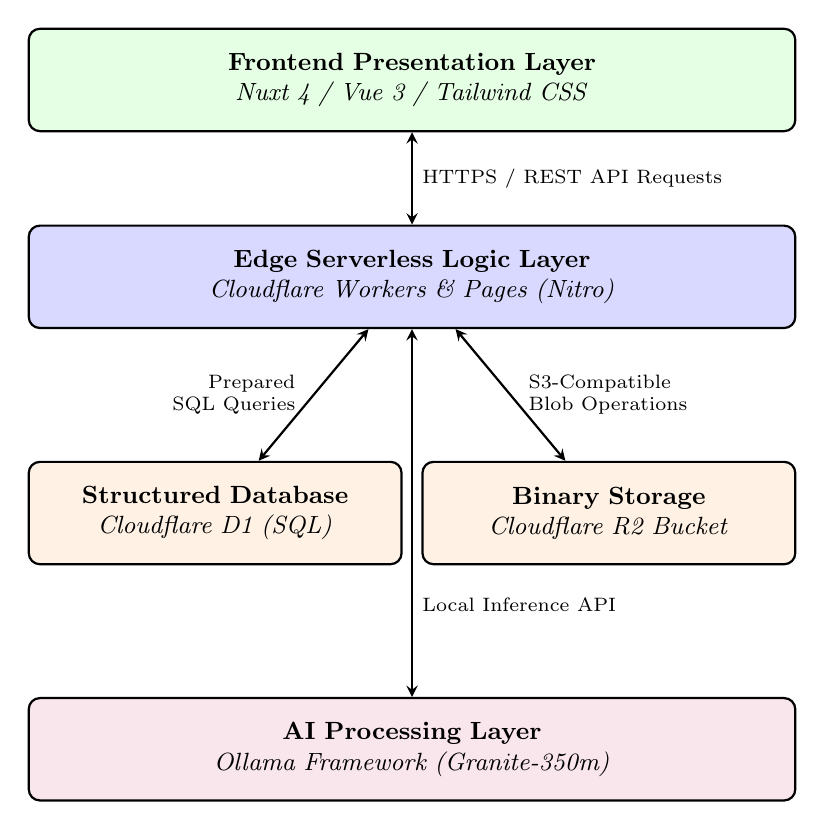
\begin{tikzpicture}[
        box/.style={rectangle, draw, rounded corners, align=center, font=\small, thick},
        bidirectional/.style={draw, <->, >=stealth, thick}
    ]
        % Nodes
        \node [box, fill=green!10, text width=9.5cm, minimum height=1.3cm] (client) at (0, 0) {\textbf{Frontend Presentation Layer}\\ \textit{Nuxt 4 / Vue 3 / Tailwind CSS}};
        
        \node [box, fill=blue!15, text width=9.5cm, minimum height=1.3cm] (edge) at (0, -2.5) {\textbf{Edge Serverless Logic Layer}\\ \textit{Cloudflare Workers \& Pages (Nitro)}};
        
        \node [box, fill=orange!10, text width=4.5cm, minimum height=1.3cm] (db) at (-2.5, -5.5) {\textbf{Structured Database}\\ \textit{Cloudflare D1 (SQL)}};
        
        \node [box, fill=orange!10, text width=4.5cm, minimum height=1.3cm] (storage) at (2.5, -5.5) {\textbf{Binary Storage}\\ \textit{Cloudflare R2 Bucket}};
        
        \node [box, fill=purple!10, text width=9.5cm, minimum height=1.3cm] (ai) at (0, -8.5) {\textbf{AI Processing Layer}\\ \textit{Ollama Framework (Granite-350m)}};
        
        % Connections
        \path [bidirectional] (client) -- node[right, font=\scriptsize] {HTTPS / REST API Requests} (edge);
        
        \path [bidirectional] (edge) -- node[left, font=\scriptsize, align=right, xshift=-0.1cm] {Prepared\\SQL Queries} (db);
        \path [bidirectional] (edge) -- node[right, font=\scriptsize, align=left, xshift=0.1cm] {S3-Compatible\\Blob Operations} (storage);
        
        % The line passes between db and storage, label is positioned in the empty space below them
        \path [bidirectional] (edge) -- node[right, font=\scriptsize, pos=0.75] {Local Inference API} (ai);
        
    \end{tikzpicture}
    \caption{JobNova Detailed Layered Serverless Architecture}
\end{figure}

\newpage
\section{Use Case Diagram}

The Use Case Diagram illustrates the primary interactions of the target actors (Job Seekers, Employers, and Administrators) with the key functions of the JobNova system.

\begin{figure}[H]
    \centering
    \includegraphics[width=\linewidth]{use-case-diagram.png}
    \caption{JobNova Use Case Diagram}
    \label{fig:use_case_diagram}
\end{figure}

\newpage
\section{Data Flow Diagram}

The Data Flow Diagram (DFD) illustrates the flow of information through the JobNova application. It shows how user inputs are collected by the frontend client, processed through serverless edge functions, authenticated, stored, and sent for AI processing:
\begin{itemize}
    \item \textbf{User Inputs}: Users (Job Seekers and Employers) interact with Vue components in the frontend, sending credentials, profile info, and chat messages.
    \item \textbf{Frontend File Processing}: Uploaded files (resumes, company verification documents) are converted to Base64 data URIs via the \texttt{FileReader} API before transmission.
    \item \textbf{Edge Server APIs}: The Nitro backend validates sessions and forwards requests to role-based API endpoints.
    \item \textbf{Storage and Database}: Database transactions read/write records to the Cloudflare D1 SQL database. Large files are pushed and cached in Cloudflare R2 bucket storage and accessed via the custom static file serving route.
    \item \textbf{Local AI Pipeline}: Chat messages are sent to the local Ollama LLM framework. The LLM processes conversational history for user profile extraction and candidate screening scoring, returning structured JSON or chat replies.
\end{itemize}

\begin{figure}[H]
    \centering
    \includegraphics[width=\linewidth]{data-flow-diagram.png}
    \caption{JobNova System Data Flow Diagram}
    \label{fig:data_flow_diagram}
\end{figure}

\newpage
\section{Sequence Diagram}

The Sequence Diagram details the step-by-step runtime interactions between the system actors, Nuxt Client, Nitro server backend, D1 database, and the local Ollama LLM service for the core AI operations:
\begin{itemize}
    \item \textbf{Scenario 1: AI Onboarding Chat and Profile Extraction}: Shows the user sending an onboarding message, the backend validating the session and logging the message in D1, calling the Ollama API to generate a chat reply, and concurrently launching a non-blocking background extraction prompt to parse the conversation history into a structured JSON profile stored in D1.
    \item \textbf{Scenario 2: Post-Application AI Screening}: Outlines the application screening flow, where the user responds to interview questions, the backend updates the chat history in the database, forwards the history to the LLM alongside the custom employer screening prompt, and on conclusion triggers the grading prompt to score (0--100) and summarize the candidate's performance.
\end{itemize}

\begin{figure}[H]
    \centering
    \includegraphics[width=\linewidth]{sequence-diagram.png}
    \caption{JobNova AI System Sequence Diagram}
    \label{fig:sequence_diagram}
\end{figure}

\newpage
\section{Class Diagram}

The Class Diagram illustrates the object-oriented structure of the core data entities within the JobNova application. It defines the attributes, methods, and relationships between primary entities such as User, JobSeekerProfile, EmployerProfile, Job, and JobApplication.

\begin{figure}[H]
    \centering
    \includegraphics[width=\linewidth, height=20cm]{class-diagram.png}
    \caption{JobNova Class Diagram}
    \label{fig:class_diagram}
\end{figure}

\newpage
\section{Deployment Guide}

The deployment of JobNova leverages Cloudflare's serverless edge infrastructure for maximum scalability and minimal maintenance. Below are the steps and prerequisites required to deploy the application from source to production:

\subsection{Prerequisites}
\begin{itemize}[itemsep=0pt]
    \item A registered \textbf{Cloudflare Account}.
    \item \textbf{Bun Runtime} (v1.1+) or Node.js (v20+) installed locally.
    \item \textbf{Wrangler CLI} installed and authenticated (\texttt{npm install -g wrangler} \& \texttt{wrangler login}).
    \item A locally running instance of \textbf{Ollama} (with the \texttt{granite4:350m} model pulled).
\end{itemize}

\subsection{1. Provisioning Cloudflare Resources}
\begin{enumerate}[itemsep=0pt]
    \item \textbf{Create the D1 Database}: Run \texttt{wrangler d1 create jobnova-db}. Note the generated \texttt{database\_name} and \texttt{database\_id} to update your \texttt{wrangler.toml}.
    \item \textbf{Create the R2 Bucket}: Run \texttt{wrangler r2 bucket create jobnova-bucket}. Update the binding in \texttt{wrangler.toml}.
    \item \textbf{Run Database Migrations}: Execute \texttt{wrangler d1 execute jobnova-db --local --file=./migrations/0000\_initial.sql} for local development, or omit \texttt{--local} for production setup.
\end{enumerate}

\subsection{2. Environment Configuration}
Create a \texttt{.env} file in the root directory and configure the necessary application secrets:
\begin{lstlisting}[language=bash, caption=Sample Environment Configuration]
NUXT_SESSION_PASSWORD="your-32-character-secure-secret"
OLLAMA_URL="http://127.0.0.1:11434/api/chat"
\end{lstlisting}

\subsection{3. Building and Deploying}
The application uses the Nuxt Nitro engine to compile the Vue frontend and server API into a single Worker compatible format.
\begin{enumerate}[itemsep=0pt]
    \item \textbf{Install Dependencies}: Run \texttt{bun install} in the project root.
    \item \textbf{Local Development}: Run \texttt{bun run dev} to test the application locally with Miniflare.
    \item \textbf{Production Build}: Run \texttt{bun run build} to generate the static assets and edge functions.
    \item \textbf{Deploy to Edge}: Run \texttt{bun run deploy} (which triggers \texttt{wrangler pages deploy dist}) to push the application live across Cloudflare's global network.
\end{enumerate}


% Chapter 7: Database Design
\chapter{DATABASE DESIGN (SCHEMA)}

\section{Overview}

The database system is constructed using Cloudflare D1, an SQLite-compatible SQL database. The schema is normalized to ensure data integrity and indexed to enable fast searches for job listings, applicant histories, and chat transcripts.

\section{Entity-Relationship (ER) Schema Overview}

The schema contains eight key tables:
\begin{itemize}
    \item \textbf{users}: Manages credential authentication and system roles.
    \item \textbf{jobseeker\_profiles}: Holds personal, academic, and professional fields, along with R2 URLs.
    \item \textbf{employer\_profiles}: Stores company details, verification document URLs, and approval status.
    \item \textbf{jobs}: Contains job specs, requirements, and AI screening configurations.
    \item \textbf{job\_applications}: Maps candidates to jobs, tracking status and storing AI screening feedback.
    \item \textbf{chat\_messages}: Logs the interactive profile onboarding conversation.
    \item \textbf{agent\_messages}: Stores history for the AI Job Agent.
    \item \textbf{govt\_jobs}: Stores scraped listings of public sector opportunities.
\end{itemize}

\begin{figure}[H]
    \centering
    \includegraphics[width=\linewidth]{er-diagram.png}
    \caption{Relational Database Schema Diagram}
\end{figure}
\newpage

\section{Table Definitions}

\subsection{1. Users Table}
Stores credentials and roles.
\begin{table}[H]
\centering
\small
\begin{tabular}{|p{2.8cm}|p{2.0cm}|p{2.5cm}|p{6.7cm}|}
\hline
\textbf{Field Name} & \textbf{Data Type} & \textbf{Constraint} & \textbf{Description} \\ \hline
id & INTEGER & PRIMARY KEY, AUTOINCREMENT & Unique identifier for each user. \\ \hline
email & TEXT & UNIQUE, NOT NULL & User's email address used for login. \\ \hline
password & TEXT & NOT NULL & Securely hashed user password. \\ \hline
role & TEXT & DEFAULT 'jobseeker' & Role of the user: 'jobseeker', 'employer', or 'admin'. \\ \hline
created\_at & TEXT & DEFAULT (datetime('now')) & Timestamp of account creation. \\ \hline
updated\_at & TEXT & DEFAULT (datetime('now')) & Timestamp of last profile update. \\ \hline
\end{tabular}
\caption{Users Table Schema}
\end{table}

\newpage 

\subsection{2. Job Seeker Profiles Table}
Tracks candidate metadata and unstructured info.
\begin{table}[H]
\centering
\small
\begin{tabular}{|p{2.8cm}|p{2.0cm}|p{2.5cm}|p{6.7cm}|}
\hline
\textbf{Field Name} & \textbf{Data Type} & \textbf{Constraint} & \textbf{Description} \\ \hline
id & INTEGER & PRIMARY KEY, AUTOINCREMENT & Unique profile identifier. \\ \hline
user\_id & INTEGER & UNIQUE, REFERENCES users(id) & Foreign key linking to the user account. \\ \hline
full\_name & TEXT & - & Full name of the job seeker. \\ \hline
phone & TEXT & - & Contact phone number. \\ \hline
location & TEXT & - & Geographical location of the candidate. \\ \hline
about\_self & TEXT & - & Short self-introduction/about text. \\ \hline
academic\_info & TEXT & - & JSON array representing academic records (degree, institution, etc.). \\ \hline
professional\_info & TEXT & - & JSON array representing work experience (company, role, duration). \\ \hline
skills & TEXT & - & Comma-separated list of candidate skills. \\ \hline
resume\_url & TEXT & - & Cloudflare R2 URL of the uploaded resume PDF. \\ \hline
resume\_name & TEXT & - & Filename of the uploaded resume. \\ \hline
completeness\_score & INTEGER & DEFAULT 0 & Score tracking profile completeness (0--100). \\ \hline
\end{tabular}
\caption{Job Seeker Profiles Table Schema}
\end{table}

\newpage

\subsection{3. Employer Profiles Table}
Tracks company registrations and admin verification.
\begin{table}[H]
\centering
\small
\begin{tabular}{|p{2.8cm}|p{2.0cm}|p{2.5cm}|p{6.7cm}|}
\hline
\textbf{Field Name} & \textbf{Data Type} & \textbf{Constraint} & \textbf{Description} \\ \hline
id & INTEGER & PRIMARY KEY, AUTOINCREMENT & Unique employer profile identifier. \\ \hline
user\_id & INTEGER & UNIQUE, REFERENCES users(id) & Foreign key linking to the user account. \\ \hline
company\_name & TEXT & - & Registered name of the organization. \\ \hline
company\_type & TEXT & - & Type of organization (e.g. Private, Public, Govt). \\ \hline
industry\_type & TEXT & - & Sector classification (e.g. IT, Finance, Retail). \\ \hline
executive\_name & TEXT & - & Name of company representative. \\ \hline
executive\_phone & TEXT & - & Contact number of company representative. \\ \hline
address & TEXT & - & Detailed postal address of the company. \\ \hline
city & TEXT & - & City location. \\ \hline
state & TEXT & - & State location. \\ \hline
pincode & TEXT & - & Postal pincode. \\ \hline
is\_approved & INTEGER & DEFAULT 0 & Verification status (0 = Pending, 1 = Approved). \\ \hline
logo\_url & TEXT & - & Cloudflare R2 URL of the company logo. \\ \hline
verification\_document\_url & TEXT & - & Cloudflare R2 URL of verification proof. \\ \hline
\end{tabular}
\caption{Employer Profiles Table Schema}
\end{table}

\newpage

\subsection{4. Jobs Table}
Stores private job vacancies.
\begin{table}[H]
\centering
\small
\begin{tabular}{|p{2.8cm}|p{2.0cm}|p{2.5cm}|p{6.7cm}|}
\hline
\textbf{Field Name} & \textbf{Data Type} & \textbf{Constraint} & \textbf{Description} \\ \hline
id & INTEGER & PRIMARY KEY, AUTOINCREMENT & Unique job listing identifier. \\ \hline
employer\_id & INTEGER & REFERENCES users(id) & Foreign key linking to the posting employer. \\ \hline
title & TEXT & NOT NULL & Job role/title. \\ \hline
functional\_area & TEXT & NOT NULL & Functional area of the job (e.g. software development). \\ \hline
industry & TEXT & NOT NULL & Industry category. \\ \hline
description & TEXT & NOT NULL & Comprehensive job description. \\ \hline
vacancies & INTEGER & DEFAULT 1 & Number of available vacancies. \\ \hline
exp\_min & INTEGER & - & Minimum experience required in years. \\ \hline
exp\_max & INTEGER & - & Maximum experience required in years. \\ \hline
sal\_min & INTEGER & - & Minimum salary offered. \\ \hline
sal\_max & INTEGER & - & Maximum salary offered. \\ \hline
city & TEXT & - & City location of the posting. \\ \hline
state & TEXT & - & State location. \\ \hline
is\_msme & INTEGER & DEFAULT 0 & Flag indicating if the employer is an MSME (0 or 1). \\ \hline
ai\_screening\_enabled & INTEGER & DEFAULT 0 & Flag indicating if AI screening is enabled (0 or 1). \\ \hline
ai\_screening\_prompt & TEXT & - & Custom prompt instructions for the AI screener. \\ \hline
\end{tabular}
\caption{Jobs Table Schema}
\end{table}



% Chapter 8: IMPLEMENTATION DETAILS
\chapter{IMPLEMENTATION DETAILS}

\section{Backend Services}

The backend logic is implemented as modular event handlers inside Nuxt's server routes directory (`/server/api`). These handlers execute on Cloudflare Workers edge.
\begin{itemize}
    \item \textbf{Database Client}: Utilizes the native Cloudflare D1 SQL client. Prepared statements are used for all queries to ensure execution efficiency and prevent SQL injection.
    \item \textbf{File Storage Operations}: Integrates with the Cloudflare R2 bucket via the S3-compatible binding API. Files (company registration proofs, resumes) are directly uploaded and referenced by URL.
    \item \textbf{Authentication Handler}: Implements JWT tokens or secure session cookies to enforce role-based access control (RBAC). Middleware interceptors block unauthorized access to employer dashboards.
\end{itemize}

\section{Frontend Application}

The client-side application is built using Nuxt 4 and Vue 3.
\begin{itemize}
    \item \textbf{State Management}: Uses Vue composables to manage user authentication, session persistence, and reactive chat logging.
    \item \textbf{Styling}: Employs a custom design system implemented via Tailwind CSS. The color scheme revolves around HSL-derived Nova Blue (\#1A73E8) and Slate Grays.
    \item \textbf{Typography}: Headings are styled in Hanken Grotesk for a modern startup aesthetic, while body text uses Inter to ensure legibility in data-dense candidate lists.
\end{itemize}

\section{AI Integration and Prompt Engineering}

The conversational logic connects to Ollama, running a localized model (`granite4:350m`).
\begin{itemize}
    \item \textbf{Conversational Onboarding}: A system prompt instructs the model to act as a friendly HR recruiter, asking one question at a time to gather personal, educational, and professional history. Upon completion, a separate prompt instructs the LLM to parse the message history and output a structured JSON schema containing the user profile.
    \item \textbf{AI Screening Chat}: When a candidate applies for an AI-enabled job, the system initiates a chat using the employer's screening prompt. The LLM conducts a structured interview. When the chat ends, the backend triggers an evaluation prompt, commanding the model to grade the candidate (0-100) and write a summary.
    \item \textbf{AI Job Agent}: A chat loop where the LLM parses user queries, matches skills with job requirements, and provides career advice.
\end{itemize}

\section{Security Measures}
\begin{itemize}
    \item \textbf{Password Hashing}: Passwords are securely hashed using standard cryptographic functions before database storage.
    \item \textbf{Data Isolation}: Strict query parameters isolate candidate applications, ensuring employers can only view candidate records submitted to their own jobs.
    \item \textbf{Secured File Access}: Uploads to Cloudflare R2 are filtered by mime-types (allowing only PDFs for resumes, and PNGs/JPGs for logos) to prevent malicious executions.
\end{itemize}


% Chapter 9: SYSTEM SPECIFICATION
\chapter{SYSTEM SPECIFICATION}

\section{Software Requirements}

\subsection{Development Environment}
\begin{itemize}
    \item \textbf{Runtime}: Bun (version 1.0+) or Node.js (version 18+)
    \item \textbf{Package Manager}: Bun (preferred as per project guidelines)
    \item \textbf{Framework}: Nuxt 4 (Vue 3, TypeScript, Tailwind CSS)
    \item \textbf{AI Hosting}: Ollama API hosting the \texttt{granite4:350m} model
\end{itemize}

\subsection{Cloud Infrastructure}
\begin{itemize}
    \item \textbf{Hosting Platform}: Cloudflare Pages
    \item \textbf{Database System}: Cloudflare D1 (SQLite-compatible SQL)
    \item \textbf{Object Storage}: Cloudflare R2 (S3-compatible API)
    \item \textbf{Tooling}: Cloudflare Wrangler CLI for local development, database migrations, and edge deployment
\end{itemize}

\section{Hardware Requirements}

\subsection{Development Machine}
\begin{itemize}
    \item \textbf{Processor}: Quad-core Intel i5/AMD Ryzen 5 minimum (Hexa-core recommended)
    \item \textbf{RAM}: 16 GB minimum (to run local Ollama models concurrently with the dev server)
    \item \textbf{Storage}: 20 GB free SSD storage
\end{itemize}

\subsection{Client Devices}
\begin{itemize}
    \item Any modern smartphone, tablet, or desktop with an HTML5-compliant web browser.
    \item \textbf{Network}: Stable internet connection for API exchanges.
\end{itemize}


% Chapter 10: VISUAL TOUR
\chapter{VISUAL TOUR (SCREENSHOTS)}

\section{Account Selection and Authentication}
The user is presented with a choice to register as a job seeker or an employer. The clean, professional landing page features a minimalist input form for login.

\begin{figure}[H]
    \centering
    \includegraphics[width=0.85\textwidth]{screenshots/index.png}
    \caption{JobNova Landing Page / Homepage}
    \label{fig:screenshot_index}
\end{figure}

\begin{figure}[H]
    \centering
    \includegraphics[width=0.85\textwidth]{screenshots/register-choose-account-type.png}
    \caption{Account Registration Role Selection}
    \label{fig:screenshot_register_choose}
\end{figure}

\begin{figure}[H]
    \centering
    \includegraphics[width=0.85\textwidth]{screenshots/login.png}
    \caption{User Login Page}
    \label{fig:screenshot_login}
\end{figure}

\section{AI Profile Builder Chat}
When job seekers sign up, they are guided by the AI recruiter chatbot. Instead of a long form, they answer questions in a conversational panel, and their details are progressively extracted.

\begin{figure}[H]
    \centering
    \includegraphics[width=0.85\textwidth]{screenshots/register-job-seeker-chat.png}
    \caption{AI Conversational Onboarding for Job Seekers}
    \label{fig:screenshot_register_chat}
\end{figure}

\section{Job Seeker Dashboard and AI Job Agent}
The main portal for candidates displays personalized job listings, application statuses, and a panel for the conversational AI Job Agent, which answers questions and processes applications.

\begin{figure}[H]
    \centering
    \includegraphics[width=0.85\textwidth]{screenshots/jobseeker-dashboard.png}
    \caption{Job Seeker Dashboard and Profiles Overview}
    \label{fig:screenshot_jobseeker_dashboard}
\end{figure}

\begin{figure}[H]
    \centering
    \includegraphics[width=0.85\textwidth]{screenshots/job-agent.png}
    \caption{Conversational AI Job Agent Interface}
    \label{fig:screenshot_job_agent}
\end{figure}

\begin{figure}[H]
    \centering
    \includegraphics[width=0.85\textwidth]{screenshots/job-search.png}
    \caption{Job Search Engine with Advanced Filters}
    \label{fig:screenshot_job_search}
\end{figure}

\begin{figure}[H]
    \centering
    \includegraphics[width=0.85\textwidth]{screenshots/job-screening-chat.png}
    \caption{AI Interview Screening Chat for Candidates}
    \label{fig:screenshot_job_screening}
\end{figure}

\section{Employer Dashboard and Applicant Tracking}
Employers can view their job listings, candidate details, R2 uploaded documents, and AI-generated screening scores and summaries, helping them identify qualified leads.

\begin{figure}[H]
    \centering
    \includegraphics[width=0.85\textwidth]{screenshots/applicants-tracking-employer-dashboard.png}
    \caption{Employer Dashboard: Candidate Applications with AI Screening Scores}
    \label{fig:screenshot_applicants_tracking}
\end{figure}

\begin{figure}[H]
    \centering
    \includegraphics[width=0.85\textwidth]{screenshots/post-a-new-job-employer-dashboard.png}
    \caption{Employer Dashboard: Job Post Creator with AI Screening Configurations}
    \label{fig:screenshot_post_job}
\end{figure}

\section{Government Jobs Portal}
The platform also aggregates public sector jobs, allowing users to view details for listings like SSC CGL directly within JobNova.

\begin{figure}[H]
    \centering
    \includegraphics[width=0.85\textwidth]{screenshots/government-jobs.png}
    \caption{Unified Government Jobs Feed (Scraped Openings)}
    \label{fig:screenshot_government_jobs}
\end{figure}

\begin{figure}[H]
    \centering
    \includegraphics[width=0.85\textwidth]{screenshots/ssc-cgl-2026-details.png}
    \caption{Government Job Details View (Scraped Info)}
    \label{fig:screenshot_gov_details}
\end{figure}


% Chapter 11: MODULES DESCRIPTION
\chapter{MODULES DESCRIPTION}

\section{Authentication and Authorization Module}
Manages security boundaries using session cookies and routing middlewares. It checks user roles on each navigation request. Job seekers are redirected away from recruiter dashboards, and unapproved recruiters are directed to a pending registration page.

\section{AI Profile Builder Module}
Handles the conversational onboarding flow. It stores message logs in the \texttt{chat\_messages} table. When the user finishes the conversation, the module sends the chat history to the local Ollama LLM, which parses and formats the personal, academic, and professional fields, updating the \texttt{jobseeker\_profiles} record.

\section{Jobs and Aggregation Module}
Manages job postings. Employers can insert, edit, or delete private job records. Concurrently, the module displays government sector jobs. A separate scraping script (\texttt{scrape-gov-jobs.py}) collects public postings (like SSC CGL) and stores them in the \texttt{govt\_jobs} table.

\section{AI Job Agent Module}
A chat component on the seeker dashboard. The AI agent acts as a career consultant. It queries active jobs in the D1 database to suggest roles matching the seeker's profile.

\section{AI Applicant Screener Module}
Initiates interviews for jobs with screening enabled. The candidate completes a text interview. When submitted, the module uses the LLM to grade the responses against the job's screening prompt, writing a candidate summary and updating the status to "Applied" with a calculated score.


% Chapter 12: DISADVANTAGES & COUNTERMEASURES
\chapter{DISADVANTAGES \& COUNTERMEASURES}

\section{Disadvantages}

\subsection{1. LLM Hallucinations and Inconsistencies}
The local model may occasionally misinterpret candidate inputs, resulting in missing information or inaccurate profile extraction.

\subsection{2. Local LLM Latency}
Running local LLMs via Ollama can introduce execution delays during high-traffic screening interviews if the host hardware lacks GPU acceleration.

\subsection{3. Fragility of the Scraping Engine}
Government job portals frequently update their HTML layouts. This can break the scraper script, resulting in missing government listings.

\subsection{4. Offline Limitations}
Since AI processing and D1 queries require active network execution, the platform has limited features when network connectivity is lost.

\section{Countermeasures}

\subsection{1. Validation and Fallbacks}
Extracted JSON profiles are validated by backend schemas. If fields are missing or invalid, the interface falls back to a standard form, allowing candidates to manually confirm and edit details.

\subsection{2. Model Quantization and Cloud Migration}
To mitigate latency, the project uses a small, optimized model (\texttt{granite4:350m}). In production environments, the AI layer can be migrated to Cloudflare Workers AI, running Llama-3 at the edge for low latency.

\subsection{3. Robust Parser Design}
The scraping script uses structured JSON outputs and falls back to searching multiple public sources. Regular updates keep the scraper aligned with target government portals.

\subsection{4. Local Storage Caching}
The frontend utilizes browser local storage to cache active chat states. This allows candidates to resume their AI onboarding or screening chats if their connection drops.


% Chapter 13: SOURCE CODE
\chapter{SOURCE CODE}

\section{Introduction}
This chapter provides the complete source code implementation for the AI Job Agent. The agent is composed of two primary components:
\begin{enumerate}
    \item \textbf{Frontend Interface (\texttt{job-agent.vue})}: A reactive, chat-based UI built in Vue 3/Nuxt 4 that handles user queries, rendering message history, and interfacing with the backend REST endpoints.
    \item \textbf{Backend REST API (\texttt{agent.post.ts})}: A serverless event handler running on Cloudflare Workers edge that integrates with a D1 database for history persistence and invokes a local Ollama model with tool-calling capabilities to perform jobs searching, details retrieval, and auto-applying.
\end{enumerate}

\section{Frontend View component (\texttt{job-agent.vue})}
Below is the full Vue 3 component code managing the user interface, keyboard handlers, and local state management for the AI Job Agent.

\begin{lstlisting}[language=HTML, caption=Frontend AI Job Agent View (job-agent.vue)]
<script setup lang="ts">
import { ref, onMounted, nextTick } from 'vue'
import { useRouter } from 'vue-router'
import { useAuth } from '~/composables/useAuth'

definePageMeta({
  layout: 'jobseeker',
  hideHeader: true
})

useHead({
  title: "Job Nova - AI Job Agent",
})

const router = useRouter()
const { user, profile, fetchUser, logout } = useAuth()

interface Message {
  role: 'user' | 'assistant'
  content: string
}

const messages = ref<Message[]>([])
const inputText = ref('')
const isLoading = ref(false)
const chatContainerRef = ref<HTMLElement | null>(null)
const inputRef = ref<HTMLInputElement | null>(null)

const scrollToBottom = async () => {
  await nextTick()
  if (chatContainerRef.value) {
    chatContainerRef.value.scrollTop = chatContainerRef.value.scrollHeight
  }
}

const sendMessage = async () => {
  const text = inputText.value.trim()
  if (!text || isLoading.value) return

  inputText.value = ''
  messages.value.push({ role: 'user', content: text })
  scrollToBottom()
  isLoading.value = true

  try {
    const data = await $fetch<{ reply: string }>('/api/agent', {
      method: 'POST',
      body: { message: text }
    })

    if (data) {
      messages.value.push({ role: 'assistant', content: data.reply })
    }
  } catch (err) {
    console.error('Unexpected error:', err)
    messages.value.push({ role: 'assistant', content: 'An unexpected error occurred.' })
  } finally {
    isLoading.value = false
    scrollToBottom()
    await nextTick()
    inputRef.value?.focus()
  }
}

const handleKeydown = (e: KeyboardEvent) => {
  if (e.key === 'Enter' && !e.shiftKey) {
    e.preventDefault()
    sendMessage()
  }
}

onMounted(async () => {
  if (!user.value) {
    await fetchUser()
  }
  if (!user.value) {
    router.push('/login')
    return
  }

  // Fetch initial message history
  try {
    const history = await $fetch<Message[]>('/api/agent-history')
    if (history && history.length > 0) {
        messages.value = history
    } else {
        messages.value.push({
            role: 'assistant',
            content: "Hello! I'm your AI Job Agent. I can help you find jobs, check job details, and even apply on your behalf. What kind of roles are you looking for today?"
        })
    }
  } catch (err) {
      console.error("Failed to load history", err)
  }

  await nextTick()
  inputRef.value?.focus()
})

const formatTime = () => {
    const now = new Date();
    return now.toLocaleTimeString([], { hour: '2-digit', minute: '2-digit' });
}

</script>

<template>
  <main class="flex-1 h-screen flex flex-col bg-surface relative z-10">
      <!-- Header -->
      <header class="h-[72px] shrink-0 border-b border-outline-variant/30 bg-surface-container-lowest/80 backdrop-blur-md flex items-center justify-between px-lg z-20">
        <div class="flex items-center gap-md">
          <div class="w-10 h-10 rounded-full bg-primary flex items-center justify-center shadow-sm">
            <UIcon name="i-lucide-bot" class="text-on-primary text-[20px]" />
          </div>
          <div>
            <h1 class="font-headline-sm text-headline-sm font-bold text-on-surface">AI Job Agent</h1>
            <p class="font-label-sm text-label-sm text-primary flex items-center gap-1">
              <span class="w-2 h-2 rounded-full bg-green-500 animate-pulse" /> Online
            </p>
          </div>
        </div>
        <NuxtLink to="/jobseeker-dashboard" class="text-on-surface-variant hover:text-primary transition-colors flex items-center gap-2 font-label-md text-label-md">
           <UIcon name="i-lucide-x" class="text-[20px]" /> Close
        </NuxtLink>
      </header>

      <!-- Chat Container -->
      <div ref="chatContainerRef" class="flex-1 overflow-y-auto p-lg lg:px-[15%] space-y-lg scroll-smooth pb-[100px]">
        <div v-for="(msg, index) in messages" :key="index" class="flex flex-col">

          <div v-if="msg.role === 'assistant'" class="flex items-start gap-sm">
            <div class="w-8 h-8 rounded-full bg-primary flex items-center justify-center shrink-0 mt-1">
              <UIcon name="i-lucide-bot" class="text-on-primary text-[16px]" />
            </div>
            <div class="max-w-[85%]">
              <div class="bg-surface-container-low rounded-2xl rounded-tl-sm px-md py-sm shadow-sm border border-outline-variant/20">
                <p class="font-body-md text-body-md text-on-surface whitespace-pre-wrap leading-relaxed prose prose-sm">{{ msg.content }}</p>
              </div>
              <p class="font-label-sm text-label-sm text-outline mt-xs ml-xs">
                Agent - {{ formatTime() }}
              </p>
            </div>
          </div>

          <div v-else class="flex items-end gap-sm justify-end">
            <div class="max-w-[85%]">
              <div class="bg-primary rounded-2xl rounded-br-sm px-md py-sm shadow-sm shadow-primary/20">
                <p class="font-body-md text-body-md text-on-primary whitespace-pre-wrap leading-relaxed">
                  {{ msg.content }}
                </p>
              </div>
              <p class="font-label-sm text-label-sm text-outline mt-xs mr-xs text-right">
                You - {{ formatTime() }}
              </p>
            </div>
            <div class="w-8 h-8 rounded-full bg-secondary-container flex items-center justify-center shrink-0 mt-1">
              <UIcon name="i-lucide-user" class="text-secondary text-[16px]" />
            </div>
          </div>

        </div>

        <div v-if="isLoading" class="flex items-start gap-sm">
          <div class="w-8 h-8 rounded-full bg-primary flex items-center justify-center shrink-0">
            <UIcon name="i-lucide-bot" class="text-on-primary text-[16px]" />
          </div>
          <div class="bg-surface-container-low rounded-2xl rounded-tl-sm px-md py-sm shadow-sm border border-outline-variant/20">
            <div class="flex items-center gap-xs">
              <span class="w-2 h-2 rounded-full bg-outline animate-bounce" style="animation-delay: 0ms" />
              <span class="w-2 h-2 rounded-full bg-outline animate-bounce" style="animation-delay: 150ms" />
              <span class="w-2 h-2 rounded-full bg-outline animate-bounce" style="animation-delay: 300ms" />
            </div>
          </div>
        </div>
      </div>

      <!-- Input Area -->
      <div class="p-md border-t border-outline-variant/30 bg-surface-container-lowest lg:px-[15%]">
        <div class="flex items-end gap-sm">
          <div class="flex-1 relative">
            <input
              id="agent-input"
              ref="inputRef"
              v-model="inputText"
              type="text"
              placeholder="Ask me to find jobs, show details, or apply..."
              :disabled="isLoading"
              class="w-full h-[52px] px-md bg-surface-container-low border border-outline-variant/30 rounded-xl font-body-md text-on-surface placeholder:text-outline focus:outline-none focus:border-primary focus:bg-surface-container-lowest transition-all disabled:opacity-50"
              @keydown="handleKeydown"
            >
          </div>
          <button
            :disabled="!inputText.trim() || isLoading"
            class="w-[52px] h-[52px] bg-primary text-on-primary rounded-xl flex items-center justify-center hover:bg-secondary active:scale-95 transition-all duration-150 shadow-lg shadow-primary/20 disabled:opacity-40 disabled:cursor-not-allowed shrink-0"
            @click="sendMessage"
          >
            <UIcon v-if="isLoading" name="i-lucide-loader-circle" class="text-[20px] animate-spin" />
            <UIcon v-else name="i-lucide-send-horizontal" class="text-[20px]" />
          </button>
        </div>
      </div>
    </main>
</template>

<style scoped>
body {
  font-family: "Inter", sans-serif;
}
</style>

\end{lstlisting}

\section{Backend REST Endpoint (\texttt{agent.post.ts})}
Below is the TypeScript backend handler managing Ollama tool-calling declarations, database transactions, and the final response synthesis.

\begin{lstlisting}[caption=Backend AI Job Agent API Route (agent.post.ts)]
import { defineEventHandler, readBody, createError } from 'h3'
import { getSessionUserId } from '../utils/session'

const OLLAMA_URL = process.env.OLLAMA_URL || 'http://localhost:11434/api/chat'
const MODEL = process.env.MODEL || 'gemma3:270m'

const SYSTEM_PROMPT = `You are a helpful AI Job Agent for Job Nova. You can help jobseekers find active jobs, get details about specific jobs, and apply to jobs on their behalf.
You have access to tools:
- list_jobs: Lists all active job postings. Optionally takes a search term.
- get_job_details: Gets detailed information about a specific job posting given its ID.
- apply_job: Applies to a specific job given its ID on behalf of the user.

Use the tools provided to help the user. If the user asks for a job, use list_jobs. If they want more info, use get_job_details. If they want to apply, use apply_job.
Keep your responses professional, concise, and helpful.`

interface ToolCall {
  function: {
    name: string
    arguments: Record<string, unknown>
  }
}

interface OllamaMessage {
  role: 'system' | 'user' | 'assistant' | 'tool'
  content: string
  tool_calls?: ToolCall[]
}

const tools = [
  {
    type: 'function',
    function: {
      name: 'list_jobs',
      description: 'Lists active job postings. Use this when the user is looking for jobs.',
      parameters: {
        type: 'object',
        properties: {
          search: {
            type: 'string',
            description: 'Optional search keyword to filter jobs by title, skills, or company name.'
          }
        }
      }
    }
  },
  {
    type: 'function',
    function: {
      name: 'get_job_details',
      description: 'Gets detailed information about a specific job posting. Use this when the user asks for more details about a specific job.',
      parameters: {
        type: 'object',
        properties: {
          jobId: {
            type: 'number',
            description: 'The ID of the job.'
          }
        },
        required: ['jobId']
      }
    }
  },
  {
    type: 'function',
    function: {
      name: 'apply_job',
      description: 'Applies to a specific job on behalf of the user.',
      parameters: {
        type: 'object',
        properties: {
          jobId: {
            type: 'number',
            description: 'The ID of the job to apply to.'
          }
        },
        required: ['jobId']
      }
    }
  }
]

async function callOllamaWithTools(messages: OllamaMessage[]): Promise<Record<string, any>> {
  const response = await fetch(OLLAMA_URL, {
    method: 'POST',
    headers: { 'Content-Type': 'application/json' },
    body: JSON.stringify({
      model: MODEL,
      messages,
      tools,
      stream: false,
      options: {
        temperature: 0.3
      }
    })
  })

  if (!response.ok) {
    throw new Error(`Ollama returned ${response.status}: ${await response.text()}`)
  }

  return response.json()
}

export default defineEventHandler(async (event) => {
  const { DB } = event.context.cloudflare.env as unknown as { DB: D1Database }

  const userId = getSessionUserId(event)
  if (!userId) {
    throw createError({ statusCode: 401, message: 'Not authenticated.' })
  }

  // Verify user is jobseeker
  const user = await DB
    .prepare('SELECT role FROM users WHERE id = ?')
    .bind(userId)
    .first<{ role: string }>()

  if (!user || user.role !== 'jobseeker') {
    throw createError({ statusCode: 403, message: 'Only jobseekers can use the job agent.' })
  }

  const body = await readBody(event)
  const { message } = body ?? {}

  if (!message || typeof message !== 'string' || !message.trim()) {
    throw createError({ statusCode: 400, message: 'Message cannot be empty.' })
  }

  // 1. Store user message
  await DB
    .prepare('INSERT INTO agent_messages (user_id, role, content) VALUES (?, \'user\', ?)')
    .bind(userId, message.trim())
    .run()

  // 2. Fetch history
  const historyRes = await DB
    .prepare('SELECT role, content FROM agent_messages WHERE user_id = ? ORDER BY created_at ASC')
    .bind(userId)
    .all<{ role: string, content: string }>()

  const history = historyRes.results || []

  // 3. Build messages array
  const ollamaMessages: OllamaMessage[] = [
    { role: 'system', content: SYSTEM_PROMPT },
    ...history.map(m => ({ role: m.role as 'user' | 'assistant', content: m.content }))
  ]

  let responseData
  try {
    responseData = await callOllamaWithTools(ollamaMessages)
  } catch (err) {
    console.error('Ollama error:', err)
    // To allow UI testing without actual running LLM, fake response when error occurs.
    responseData = {
      message: {
        role: 'assistant',
        content: 'Sorry, the AI service is currently down, but the endpoints have successfully been hit.'
      }
    }
  }

  let aiMessage = responseData.message as OllamaMessage

  // 4. Handle tool calls if any
  if (aiMessage.tool_calls && aiMessage.tool_calls.length > 0) {
    ollamaMessages.push(aiMessage)

    for (const toolCall of aiMessage.tool_calls) {
      const name = toolCall.function.name
      const args = toolCall.function.arguments
      let resultStr = ''

      if (name === 'list_jobs') {
        const search = args.search ? String(args.search).trim() : ''
        let sql = `SELECT j.id, j.title, j.city, ep.company_name FROM jobs j LEFT JOIN employer_profiles ep ON j.employer_id = ep.user_id WHERE j.status = 'active'`
        const params: any[] = []
        if (search) {
          sql += ' AND (j.title LIKE ? OR j.skills LIKE ? OR ep.company_name LIKE ?)'
          params.push(`%${search}%`, `%${search}%`, `%${search}%`)
        }
        sql += ' ORDER BY j.created_at DESC LIMIT 10'
        const res = await DB.prepare(sql).bind(...params).all<Record<string, unknown>>()
        resultStr = JSON.stringify(res.results || [])
      } else if (name === 'get_job_details') {
        const jobId = args.jobId
        if (jobId) {
          const sql = `SELECT j.*, ep.company_name FROM jobs j LEFT JOIN employer_profiles ep ON j.employer_id = ep.user_id WHERE j.id = ?`
          const res = await DB.prepare(sql).bind(jobId).first<Record<string, unknown>>()
          resultStr = res ? JSON.stringify(res) : JSON.stringify({ error: 'Job not found' })
        } else {
          resultStr = JSON.stringify({ error: 'jobId is required' })
        }
      } else if (name === 'apply_job') {
        const jobId = args.jobId
        if (jobId) {
          // Check if active
          const job = await DB.prepare('SELECT id, status FROM jobs WHERE id = ?').bind(jobId).first<{ id: number, status: string }>()
          if (!job || job.status !== 'active') {
            resultStr = JSON.stringify({ error: 'Job not found or not active.' })
          } else {
            // Check if already applied
            const existing = await DB.prepare('SELECT id FROM job_applications WHERE job_id = ? AND jobseeker_id = ?').bind(jobId, userId).first()
            if (existing) {
              resultStr = JSON.stringify({ error: 'You have already applied for this job.' })
            } else {
              const res = await DB.prepare('INSERT INTO job_applications (job_id, jobseeker_id, status) VALUES (?, ?, \'applied\')').bind(jobId, userId).run()
              if (res.success) {
                resultStr = JSON.stringify({ success: true, message: 'Application submitted successfully.' })
              } else {
                resultStr = JSON.stringify({ error: 'Failed to apply' })
              }
            }
          }
        } else {
          resultStr = JSON.stringify({ error: 'jobId is required' })
        }
      } else {
        resultStr = JSON.stringify({ error: 'Unknown function' })
      }

      ollamaMessages.push({
        role: 'tool',
        content: resultStr
      })
    }

    // Call Ollama again with tool results
    try {
      const finalResponse = await callOllamaWithTools(ollamaMessages)
      aiMessage = finalResponse.message
    } catch (err) {
      console.error('Ollama error (final):', err)
      aiMessage = {
        role: 'assistant',
        content: 'Sorry, the AI service is currently down, but tool execution works.'
      }
    }
  }

  // 5. Save assistant response
  await DB
    .prepare('INSERT INTO agent_messages (user_id, role, content) VALUES (?, \'assistant\', ?)')
    .bind(userId, aiMessage.content || '')
    .run()

  return {
    reply: aiMessage.content || ''
  }
})

\end{lstlisting}




% Chapter 15: CONCLUSION & FUTURE SCOPE
\chapter{CONCLUSION \& FUTURE SCOPE}

\section{Conclusion}

JobNova successfully addresses the inefficiencies of traditional recruitment systems by providing an AI-driven, serverless recruitment platform. Through conversational onboarding, automated job screening, and a unified private/government jobs portal, the platform:
\begin{itemize}
    \item Automates candidate pre-screening, reducing recruiter overhead.
    \item Enhances profile accuracy by extracting structured details through natural chat.
    \item Provides a unified search engine for Indian job seekers.
    \item Delivers high availability and low latency via Cloudflare Pages and D1.
\end{itemize}

This project demonstrates how serverless edge infrastructure and local LLM models can be combined to build a cost-effective, intelligent, and scalable recruitment platform.

\section{Future Scope}

While the current version provides a strong foundation, several enhancements can be integrated:
\begin{itemize}
    \item \textbf{Integration with Cloudflare Workers AI}: Move from local Ollama hosting to serverless LLM edge workers, running Llama-3 globally.
    \item \textbf{Direct Resume Document Parsing}: Implement file parsers (PDF/Docx) to let candidates upload resumes first, pre-seeding the AI chat profile.
    \item \textbf{Regional Language Support}: Support conversational interviews in Hindi and other regional Indian languages to make the platform accessible to a wider demographic.
    \item \textbf{Voice-Based Screening}: Integrate speech-to-text APIs to allow candidates to speak their answers during the AI screening phase.
\end{itemize}


% Chapter 16: REFERENCES
\chapter{REFERENCES}

\section{Frameworks and Libraries}
\begin{itemize}
    \item \textbf{Nuxt 4}, Online / GitHub. URL: \url{https://nuxt.com}
    \item \textbf{Vue 3}, Online. URL: \url{https://vuejs.org}
    \item \textbf{Tailwind CSS}, Online. URL: \url{https://tailwindcss.com}
    \item \textbf{Ollama}, Local / GitHub. URL: \url{https://ollama.com}
    \item \textbf{Granite / Gemma Models}, Ollama Model Library. URL: \url{https://ollama.com/library}
\end{itemize}

\section{Databases and Storage}
\begin{itemize}
    \item \textbf{Cloudflare D1}, Cloudflare Serverless Platform. URL: \url{https://developers.cloudflare.com/d1/}
    \item \textbf{Cloudflare R2}, Cloudflare Storage Platform. URL: \url{https://developers.cloudflare.com/r2/}
\end{itemize}

\section{Development Tools}
\begin{itemize}
    \item \textbf{Bun Runtime}, Local / Online. URL: \url{https://bun.sh}
    \item \textbf{Wrangler CLI}, npm registry. URL: \url{https://developers.cloudflare.com/workers/wrangler/}
    \item \textbf{Git Version Control}, Distributed System. URL: \url{https://git-scm.com}
\end{itemize}


% Chapter 17: APPENDIX
\chapter{APPENDIX}

\section{Database Table Schemas}
The database schema for JobNova is structured into relational tables in Cloudflare D1. The database includes the \texttt{users} table for credentials, \texttt{jobseeker\_profiles} for personal details, academic history, and work experience, \texttt{employer\_profiles} for verified organizations, \texttt{jobs} for private listings, \texttt{job\_applications} for candidate applications with AI evaluation scores, \texttt{chat\_messages} and \texttt{agent\_messages} for storing AI chat interactions, and \texttt{govt\_jobs} for crawled public sector announcements.


\section{AI Parsing Endpoint Handler (Nuxt Server Route)}

\begin{lstlisting}[language=HTML, caption=Sample Nuxt Server Route calling Ollama API]
import { defineEventHandler, readBody } from 'h3';

export default defineEventHandler(async (event) => {
  const body = await readBody(event);
  const messages = body.messages;

  // Make request to local Ollama API running Granite model
  const response = await fetch('http://127.0.0.1:11434/api/chat', {
    method: 'POST',
    headers: { 'Content-Type': 'application/json' },
    body: JSON.stringify({
      model: 'granite4:350m',
      messages: messages,
      stream: false
    })
  });
  
  const data = await response.json();
  return data.message;
});
\end{lstlisting}

\vfill

\begin{center}
\rule{0.5\textwidth}{0.5pt}\\
\vspace{0.5cm}
\textit{End of Project Report}\\
\vspace{0.2cm}
\textbf{JobNova}\\
\textit{AI-Powered Recruitment and Job Matching Ecosystem}
\end{center}

\end{document}
